\subsubsection{Authentification et Gestion de Compte}

Ce module assure l'authentification sécurisée via identifiants classiques ou OAuth 2.0 (Google, GitHub) avec gestion automatique des jetons d'accès. Lors de la première connexion, le système impose un changement de mot de passe pour les comptes créés par un administrateur. Un processus de réinitialisation obligatoire bloque l'accès à l'application jusqu'à la définition d'un mot de passe personnel, garantissant que seul l'utilisateur légitime détient les informations d'authentification définitives.

\begin{figure}[H]
    \centering
    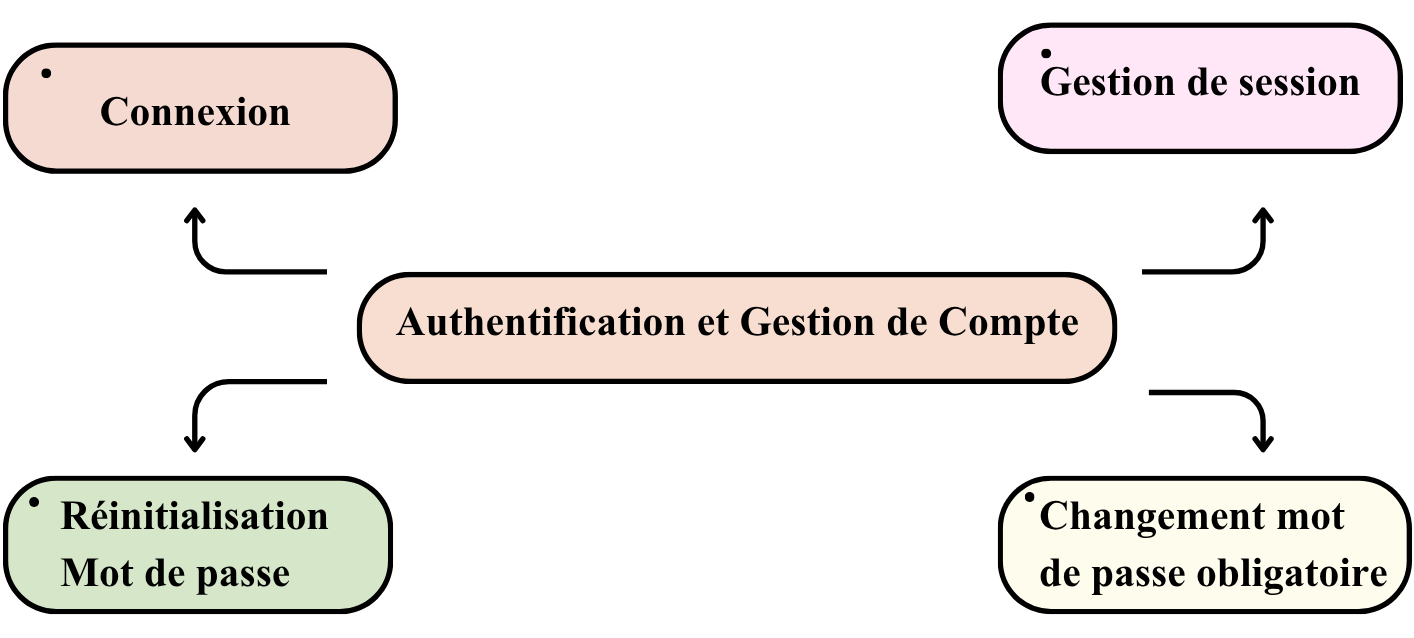
\includegraphics[width=0.7\textwidth,keepaspectratio]{Images/soumission_demande_inscription.png}
    \caption{Authentification et Gestion de Compte}
    \label{fig:authentification_gestion_compte}
\end{figure}

\vspace{0.5cm}

\subsubsection{Gestion des Utilisateurs et Demandes d'Inscription}

Ce module permet aux administrateurs de gérer le cycle de vie complet des comptes utilisateurs avec création automatisée, gestion des profils et contrôle des activations/désactivations. Le traitement des demandes d'inscription s'effectue via une interface centralisée permettant approbation, rejet ou mise en attente avec notifications automatiques.

\begin{figure}[H]
    \centering
    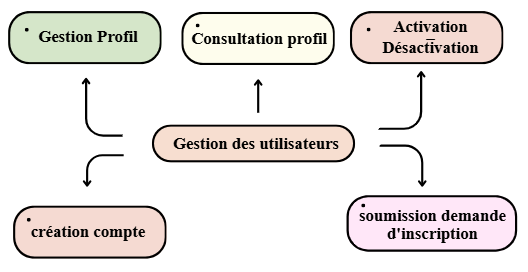
\includegraphics[width=0.7\textwidth,keepaspectratio]{Images/inscription_creation_utilisateur.png}
    \caption{Gestion des Utilisateurs et Demandes d'Inscription}
    \label{fig:gestion_utilisateurs}
\end{figure}

\vspace{0.5cm}

\subsubsection{Système de Rôles et Permissions}

Les droits sont gérés par rôles selon un modèle RBAC (Role-Based Access Control) : chaque rôle regroupe un ensemble de permissions, ce qui permet d’attribuer finement les accès. La conception modulaire permet aux administrateurs de créer des rôles personnalisés en combinant dynamiquement les permissions existantes selon les besoins organisationnels spécifiques. Cette flexibilité permet d'ajuster les autorisations d'un rôle sans impact sur les autres configurations, facilitant l'évolution du système de sécurité.

\begin{figure}[H]
    \centering
    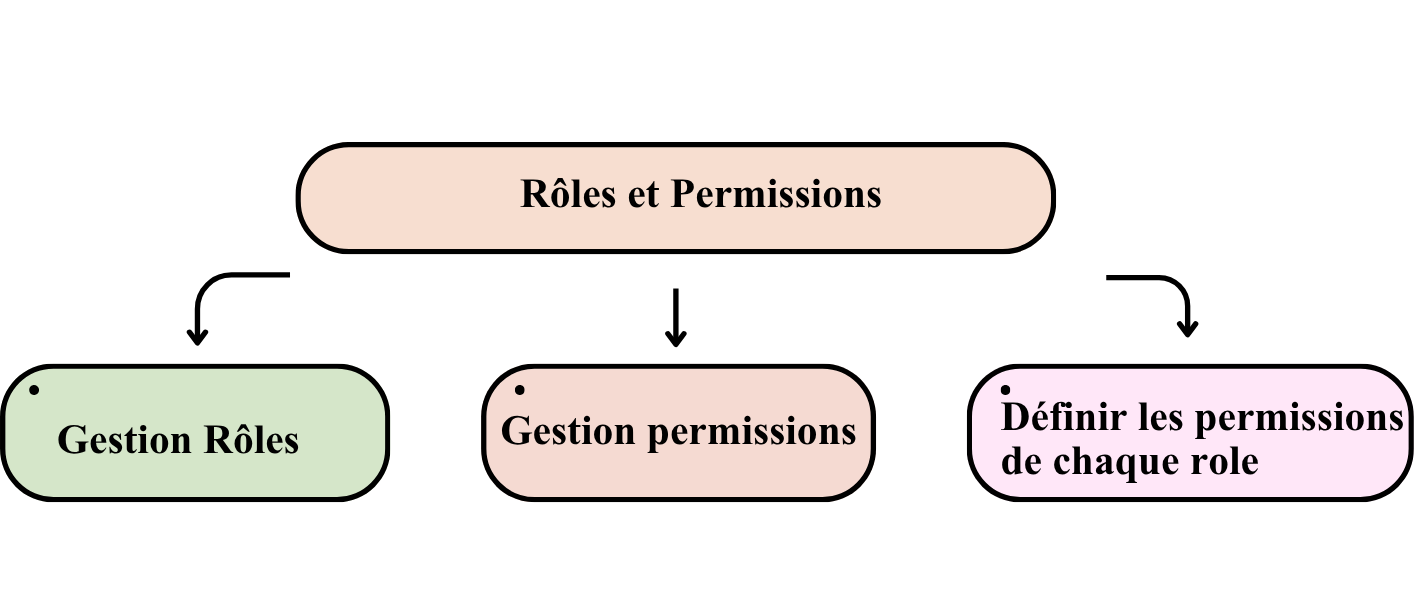
\includegraphics[width=0.7\textwidth,keepaspectratio]{Images/gestion_permissions.png}
    \caption{Système de Rôles et Permissions}
    \label{fig:roles_permissions}
\end{figure}

\vspace{0.5cm} 

\subsubsection{Gestion des Clients et Projets}

Ce module centralise la gestion des clients avec création automatisée des comptes. Le système génère des organigrammes visuels et interactifs pour chaque projet, présentant la hiérarchie complète (client, chef de projet, équipe) avec accès direct aux coordonnées de tous les interlocuteurs. Cette visualisation facilite l'identification rapide des contacts et optimise la communication en cas de problème.

\begin{figure}[H]
    \centering
    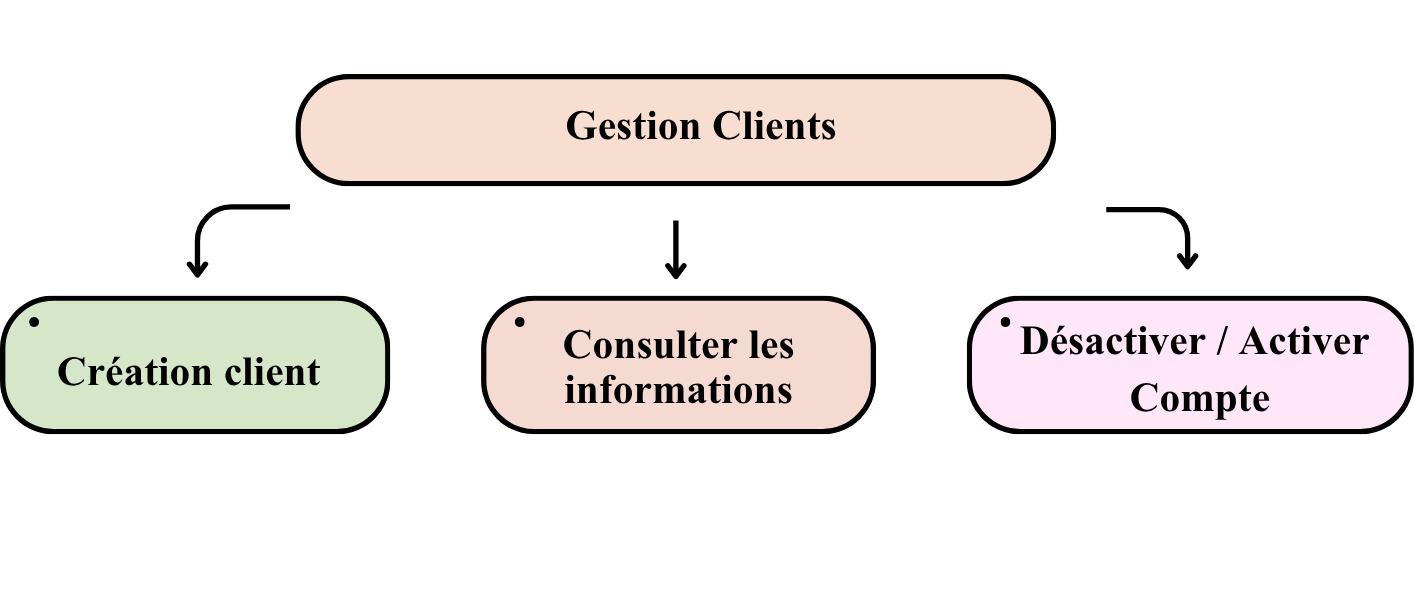
\includegraphics[width=0.7\textwidth,keepaspectratio]{Images/gestion_client.png}
    \caption{Gestion des Clients et Projets}
    \label{fig:gestion_clients}
\end{figure}

\subsubsection{Gestion des Contrats de Maintenance}

Ce module automatise le cycle de vie complet des contrats de maintenance avec système d'alertes préventives échelonnées. L'import de contrats s'effectue à partir de fichiers PDF, avec extraction automatique de données pour pré-remplir les formulaires de création.
\begin{figure}[H]
    \centering
    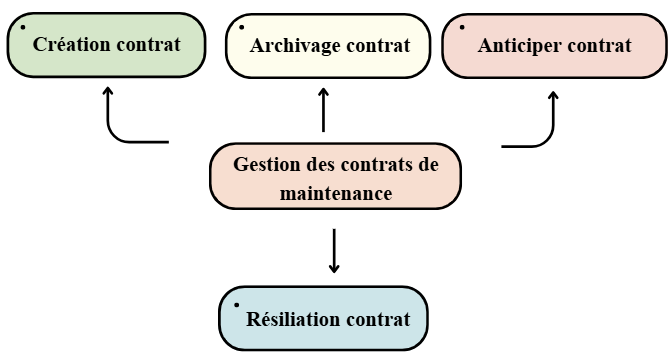
\includegraphics[width=0.7\textwidth,keepaspectratio]{Images/gestion_contrat.png}
    \caption{Gestion des contrats de maintenance}
    \label{fig:gestion_contrats}
\end{figure}

\subsubsection{Gestion des Demandes d'Intervention}

Ce module structure la soumission des demandes d'intervention avec vérification automatique de couverture contractuelle et validation des types d'intervention éligibles. Le processus de validation intègre un système de relance automatique garantissant le traitement dans les délais impartis avec escalade vers les responsables en cas de dépassement des seuils temporels.

\begin{figure}[H]
    \centering
    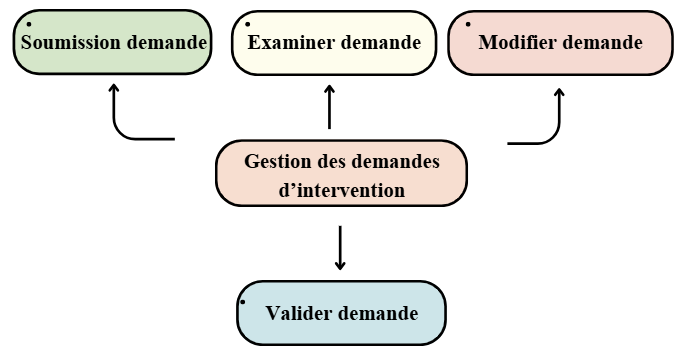
\includegraphics[width=0.7\textwidth,keepaspectratio]{Images/gestion_demande.png}
    \caption{Gestion des demandes d'intervention}
    \label{fig:gestion_demandes}
\end{figure}

\subsubsection{Gestion Avancée des Tickets de Maintenance}

Ce module recommande automatiquement les développeurs les plus adaptés à un ticket, permet de suivre le temps de travail via chronométrage, et de signaler des blocages avec analyse automatique par IA. Les solutions sont proposées collaborativement entre membres de l'équipe. La soumission en revue déclenche la clôture automatique des sessions et le calcul du temps cumulé. Après validation par le chef de projet, le client peut fermer le ticket, signaler un problème persistant, ou obtenir une extension automatique de sept jours.
\subsubsection{Tableaux de Bord, Traçabilité et Documentation}

Ce module offre des tableaux de bord personnalisés par rôle avec indicateurs clés de performance. Il maintient un historique exhaustif de toutes les opérations avec traçabilité complète et système de notifications multicanaux (web, email, Slack). La génération automatique de procès-verbaux PDF s'effectue à partir des informations de tickets lors de la résolution, produisant une documentation contractuelle structurée.

\begin{figure}[H]
    \centering
    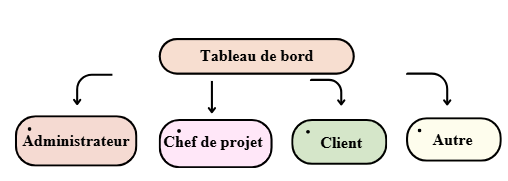
\includegraphics[width=0.7\textwidth,keepaspectratio]{Images/dashboard.png}
    \caption{Tableau de bord et reportage}
    \label{fig:dashboard}
\end{figure}

\begin{figure}[H]
    \centering
    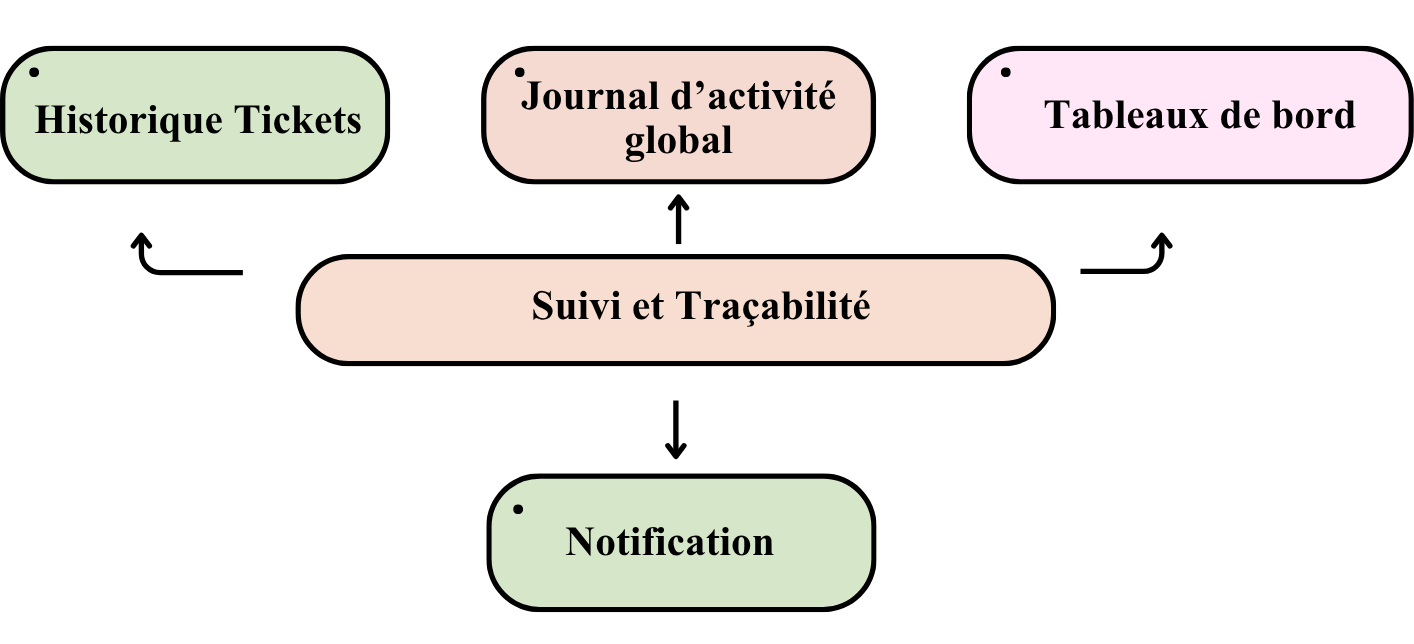
\includegraphics[width=0.7\textwidth,keepaspectratio]{Images/suivi_tracabilite.png}
    \caption{Suivi et Traçabilité}
    \label{fig:suivi_tracabilite}
\end{figure}

\begin{figure}[H]
    \centering
    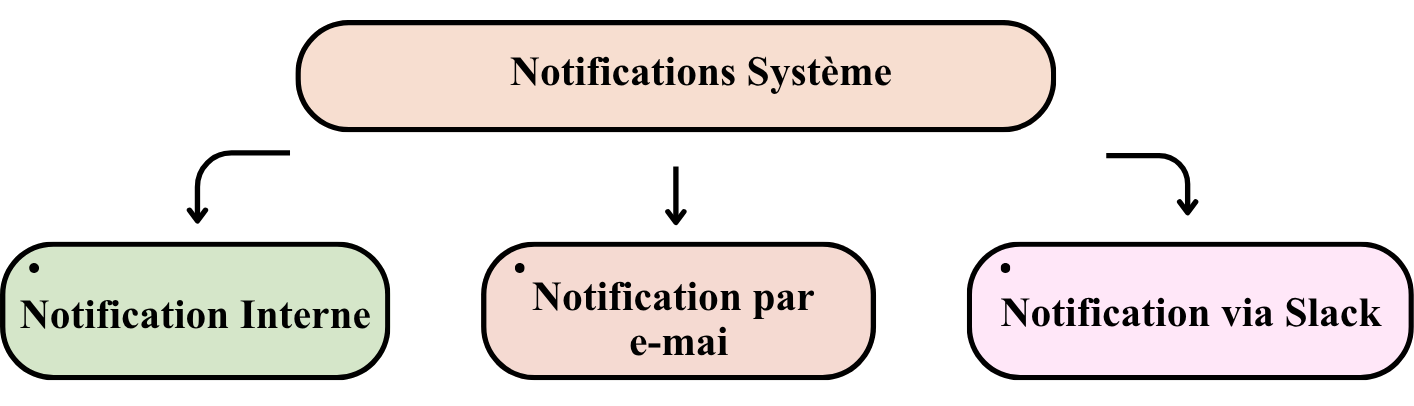
\includegraphics[width=0.7\textwidth,keepaspectratio]{Images/notifications.png}
    \caption{Notifications Système}
    \label{fig:notifications}
\end{figure}